\documentclass[addpoints]{exam}

\printanswers
\CorrectChoiceEmphasis{\color{red}\bfseries}
\usepackage{amssymb, amsmath, amsfonts}
\usepackage{geometry}
\usepackage{graphicx}
\usepackage{tikz}
\usetikzlibrary{calc}
\usepackage{multirow,array} % for payoff matrix formatting
\usepackage[colorlinks,pdfusetitle,urlcolor=blue,citecolor=blue,linkcolor=blue]{hyperref}

\definecolor{crimson}{RGB}{ 170, 4, 36 }
\definecolor{darkblue}{RGB}{ 4, 47, 170 }
\definecolor{brown}{RGB}{ 111, 71, 2 }
\definecolor{periwinkle}{RGB}{ 90, 177, 204 }
\definecolor{ducksgreen}{HTML}{007030}

\geometry{left=1.0in,right=1.0in,top=1.0in,bottom=1.0in}
\pagestyle{headandfoot}
\lhead{EC327 Game Theory}
\chead{Homework 4}
\rhead{Fall 2025}
\runningheadrule

\title{
    \textbf{Econ 327: Game Theory} \\ 
    Homework $\#4$
    }
\author{University of Oregon}
\date{Due: Oct. 24$^{th}$}

% exam-type question formatting
\renewcommand{\thequestion}{\textbf{Q\arabic{question}}}
\bracketedpoints

\begin{document}

\maketitle

\begin{center}
  \gradetable[h][questions]
\end{center}

\vspace{0.5in}

\begin{center}
  \textbf{For homework assignments:}
\end{center}

\begin{itemize}

%  \item DO NOT write your name:
%  this assignment will be graded anonymously. 
%  If you want to, you can include your student ID instead.

  \item Complete \textit{all} questions and parts.

  % I will select one question at random to be graded
  % according to the rubric on Canvas.

  \item You will be graded on not only the content of your work
    but on how clearly you present your ideas.
    Make sure that your handwriting is legible.
    Please use extra pages if you run out of space 
    but make sure that all parts of a question 
    are in the correct order when you submit.

  \item You may choose to work with others,
  but everyone must submit to Canvas individually.

  Please include the names of everyone who you worked with 
  below your own name.
 
\end{itemize}

\vspace{1.0in}

\makebox[.6\textwidth]{Name\enspace\hrulefill}

\vspace{0.5in}

% \begin{center}
%   \fbox{\fbox{\parbox{5.5in}{\centering
%     Answer the questions in the spaces provided on the
%     question sheets. If you run out of room for an answer,
%     continue on the back of the page or another sheet of paper.}}}
% \end{center}

\begin{questions}

\newpage

\question
Recall the gnu and croc river crossing game from Homework 2, Question 3.
Now, consider what happens if the gnu have bad eyesight and can't see where the crocs are choosing to lie in wait.

\begin{parts}
  
\part[8]
Draw out the new extensive form game.

\begin{solution}
  Either of the following extensive forms is acceptable:

  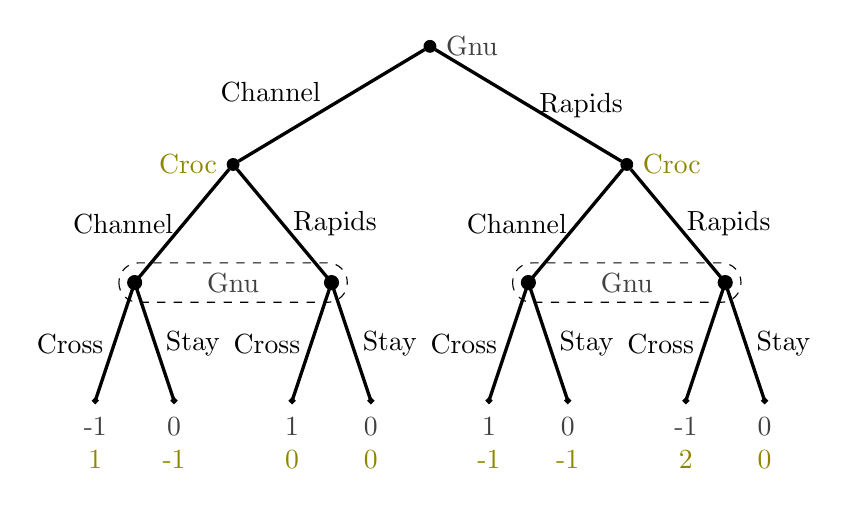
\begin{tikzpicture}[edge from parent/.style={draw, very thick}]
    \tikzstyle{solid node}=[circle,draw,inner sep=1.5,fill=black]
    \tikzstyle{hollow node}=[circle,draw,inner sep=.25]
    \tikzstyle{level 1}=[level distance=15mm,sibling distance=5cm]
    \tikzstyle{level 2}=[level distance=15mm,sibling distance=2.5cm]
    \tikzstyle{level 3}=[level distance=15mm,sibling distance=1cm]
    \tikzstyle{pruned edge from parent}=[draw, very thick, darkgray, dashed, -]
    
    \node(0)[solid node,label=right:{\color{darkgray} Gnu}]{}
        child{node[solid node,label=left:{\color{olive} Croc }]{}
            child{node(1)[solid node]{}
                child{node[hollow node,label=below:{
                    \begin{tabular}{c}
                         {\color{darkgray} -1}  \\
                         {\color{olive} 1} 
                    \end{tabular}
                }]{} edge from parent node[left]{Cross}}
                child{node[hollow node,label=below:{
                    \begin{tabular}{c}
                         {\color{darkgray} 0}  \\
                         {\color{olive} -1} 
                    \end{tabular}
                }]{} edge from parent node[right]{Stay}}
            edge from parent node[left]{Channel}}
            child{node(2)[solid node]{}
                child{node[hollow node,label=below:{
                    \begin{tabular}{c}
                         {\color{darkgray} 1}  \\
                         {\color{olive} 0} 
                    \end{tabular}
                }]{} edge from parent node[left]{Cross}}
                child{node[hollow node,label=below:{
                    \begin{tabular}{c}
                         {\color{darkgray} 0}  \\
                         {\color{olive} 0} 
                    \end{tabular}
                }]{} edge from parent node[right]{Stay}}
            edge from parent node[right]{Rapids}}
            edge from parent node[left,xshift=0,yshift=5]{Channel}
        }
        child{node[solid node,label=right:{\color{olive} Croc }]{}
            child{node(3)[solid node]{}
                child{node[hollow node,label=below:{
                    \begin{tabular}{c}
                         {\color{darkgray} 1}  \\
                         {\color{olive} -1} 
                    \end{tabular}
                }]{} edge from parent node[left]{Cross}}
                child{node[hollow node,label=below:{
                    \begin{tabular}{c}
                         {\color{darkgray} 0}  \\
                         {\color{olive} -1} 
                    \end{tabular}
                }]{} edge from parent node[right]{Stay}}
            edge from parent node[left]{Channel}}
            child{node(4)[solid node]{}
                child{node[hollow node,label=below:{
                    \begin{tabular}{c}
                         {\color{darkgray} -1}  \\
                         {\color{olive} 2} 
                    \end{tabular}
                }]{} edge from parent node[left]{Cross}}
                child{node[hollow node,label=below:{
                    \begin{tabular}{c}
                         {\color{darkgray} 0}  \\
                         {\color{olive} 0} 
                    \end{tabular}
                }]{} edge from parent node[right]{Stay}}
            edge from parent node[right]{Rapids}}
            edge from parent node[right]{Rapids}
        }
        ;
% information set
\draw[dashed,rounded corners=7]($(1)+(-.2,.25)$)rectangle($(2)+(.2,-.25)$);
\draw[dashed,rounded corners=7]($(3)+(-.2,.25)$)rectangle($(4)+(.2,-.25)$);
% specify movers
\node at ($.5*(1)+.5*(2)$) {\color{darkgray} Gnu};
\node at ($.5*(3)+.5*(4)$) {\color{darkgray} Gnu};
\end{tikzpicture}


  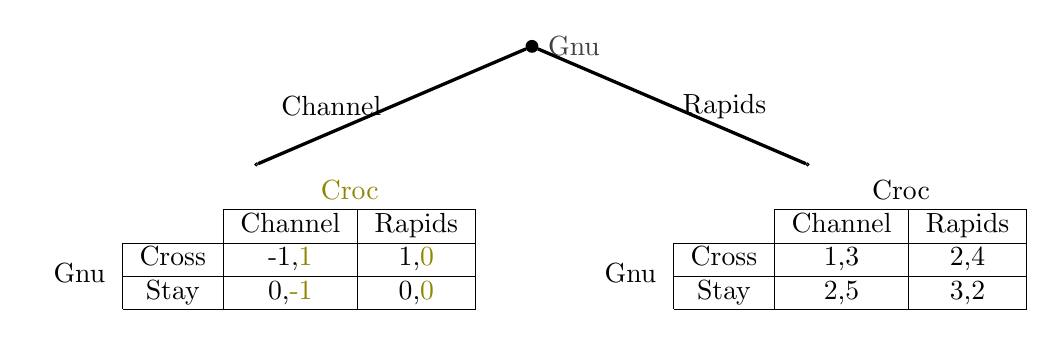
\begin{tikzpicture}[edge from parent/.style={draw, very thick}]
    \tikzstyle{solid node}=[circle,draw,inner sep=1.5,fill=black]
    \tikzstyle{hollow node}=[circle,draw,inner sep=.25]
    \tikzstyle{level 1}=[level distance=15mm,sibling distance=7cm]
    \tikzstyle{pruned edge from parent}=[draw, very thick, darkgray, dashed, -]
    
    \node(0)[solid node,label=right:{\color{darkgray} Gnu}]{}
      child{node[hollow node,label=below:{
        \begin{tabular}{*{4}{c|}}
           \multicolumn{2}{c}{} & \multicolumn{2}{c}{\color{olive} Croc} \\\cline{3-4}
           \multicolumn{1}{c}{} &       & Channel & Rapids \\\cline{2-4}
           \multirow{2}*{Gnu}   & Cross & -1,{\color{olive}1}  & 1,{\color{olive}0}   \\\cline{2-4}
                                & Stay  & 0,{\color{olive}-1}  & 0,{\color{olive}0}   \\\cline{2-4}
        \end{tabular}
      }]{}
          edge from parent node[left]{Channel}
      }
      child{node[hollow node,label=below:{
        \begin{tabular}{*{4}{c|}}
           \multicolumn{2}{c}{} & \multicolumn{2}{c}{Croc} \\\cline{3-4}
           \multicolumn{1}{c}{} &       & Channel & Rapids \\\cline{2-4}
           \multirow{2}*{Gnu}   & Cross & 1,3  & 2,4   \\\cline{2-4}
                                & Stay  & 2,5  & 3,2   \\\cline{2-4}
        \end{tabular}
      }]{}
          edge from parent node[right]{Rapids}
      }
      ;
\end{tikzpicture}

\end{solution}
  \part[4]
  How does your prediction change from homework 2?
  Would you still expect to always see the gnu safely crossing at the channel?

  \begin{solution}
    If the Gnu can't see the Crocs, they can't use a strategy where they only selectively cross the Channel if the Crocs are there.
    If they choose to Cross the Channel in this case, then the Crocs will decide it's worth it to go to the Channel.
    So the equilibrium from earlier doesn't apply because the information sets of the extensive form game have changed.
  \end{solution}

\end{parts}
\end{questions}

\end{document}
